% Chapter 3: State of the Art

\chapter{Estado del Arte} % Main chapter title

\label{Chapter3}

%-------------------------------------------------------------------------------

\section{Java}

Java es un lenguaje de programación de propósito general, orientado a objetos y concurrente. Originalmente fue desarrollado por James Gosling, Bill Joy y Guy Steele para Sun Microsystems en 1996 y fue adquirido por Oracle en 2010.

Fue diseñado para que los desarrolladores escribiesen una única vez su programa y pudieran ejecutarlo en cualquier máquina sin necesitar recompilarlo. Esto es posible debido a que las aplicaciones Java son compiladas a \emph{bytecode} que luego es ejecutado en una Java Virtual Machine (JVM), sin importar la arquitectura de la máquina. \emph{\parencite{Reference13}}

\begin{figure}[ht]
  \centering
  
\includegraphics[scale=0.3]{Figures/JavaLogo}
  \decoRule
  \caption[Java (Logo)]{Logo de Java \emph{\parencite{Reference6}}}
  \label{fig:JavaLogo}
\end{figure}

%-------------------------------------------------------------------------------

\section{Android}

\label{Android}

\keyword{Android} es un sistema operativo desarrollado por Google, basado en el \emph{kernel} de Linux.
Está diseñado principalmente para dispositivos táctiles, como \emph{smartphones} y \emph{tablets}.

Las aplicaciones de \keyword{Android} están escritas en Java.
Hasta la versión 4.4 de Android, se utilizaba Dalvik como máquina virtual con la compilación
en tiempo de ejecución (JIT) para ejecutar \emph{bytecode} Dalvik, que es una traducción del
\emph{Java bytecode}.

Android 4.4 introdujo el ART (Android Runtime) como un nuevo entorno de ejecución, que
compila el \emph{Java bytecode} durante la instalación de una aplicación. Desde Android
5.0 se convirtió en la única opción en tiempo de ejecución. \emph{\parencite{Reference7}}

\begin{figure}[ht]
  \centering
  
\includegraphics[scale=0.1]{Figures/AndroidLogo}
  \decoRule
  \caption[Android (Logo)]{Logo de Android \emph{\parencite{Reference3}}}
  \label{fig:AndroidLogo}
\end{figure}

\subsection{KeyStore}

\label{KeyStore}

El \keyword{KeyStore} de Android es un sistema que permite almacenar claves
criptográficas en un contenedor de manera que resulte más difícil extraerlas del
dispositivo.

Las claves que se encuentran en el \keyword{KeyStore} están protegidas contra la
extracción mediante dos medidas de seguridad:

\begin{itemize}
  \item En primer lugar, las claves nunca ingresan al proceso de la aplicación.
  Cuando una aplicación utiliza alguna de estas claves para llevar a cabo una
  operación criptográfica, el texto sobre el que se va a realizar la operación
  es llevado a un proceso ajeno a la aplicación que se encarga de realizar la
  operación criptográfica. De esta manera, si el proceso de la aplicación se ve
  comprometido por un atacante, este no será capaz de extraer las claves.

  \item En segundo lugar, las claves se protegen mediante hardware seguro del
  dispositivo Android. Este hardware evita que las claves puedan ser extraídas
  incluso cuando el Sistema Operativo se ve comprometido: un atacante podría
  utilizar las claves ligadas a una app para realizar operaciones
  criptográficas, pero nunca podría extraerlas del dispositivo.
\end{itemize}

\emph{\parencite{Reference33}}

%----------------------------------------------------------------------------------------

\section{Bouncy Castle}

\keyword{Bouncy Castle (BC)} es una API utilizada en criptografía.
Esta API, entre otras cosas, proporciona los siguientes servicios:
\begin{itemize}
  \item Una API criptográfica \emph{ligera} para Java y C\#.
  \item Un proveedor para Java Cryptography Extension (JCE)\footnote{JCE implementa encriptación, generación y protocolos de establecimiento de claves y algoritmos MAC.} y para Java Cryptography Architecture (JCA).
\end{itemize}

BC está mantenidos por una organización caritativa australiana, conocida como \keyword{The Legion of the Bouncy Castle}. \emph{\parencite{Reference4}}

%----------------------------------------------------------------------------------------

\section{Criptografía de clave simétrica}

La \emph{confidencialidad} en las comunicaciones es el objetivo principal que se persigue con los algoritmos de encriptación.
La \keyword{criptografía de clave simétrica} nos permite comunicarnos con otra persona (o máquina) de manera que un tercero,
aun teniendo el mensaje cifrado, no pudiera extraer nada de información de él.

Los algoritmos basados en este modelo utilizan un \emph{secreto} compartido entre los dos extremos que se quieren comunicar.
Una vez acordado, nadie que no posea este secreto podría descifrar ningún mensaje enviado por uno u otro extremo.
(Figura~\ref{fig:SymmetricKeyEncryption})

\begin{figure}[ht]
  \centering
  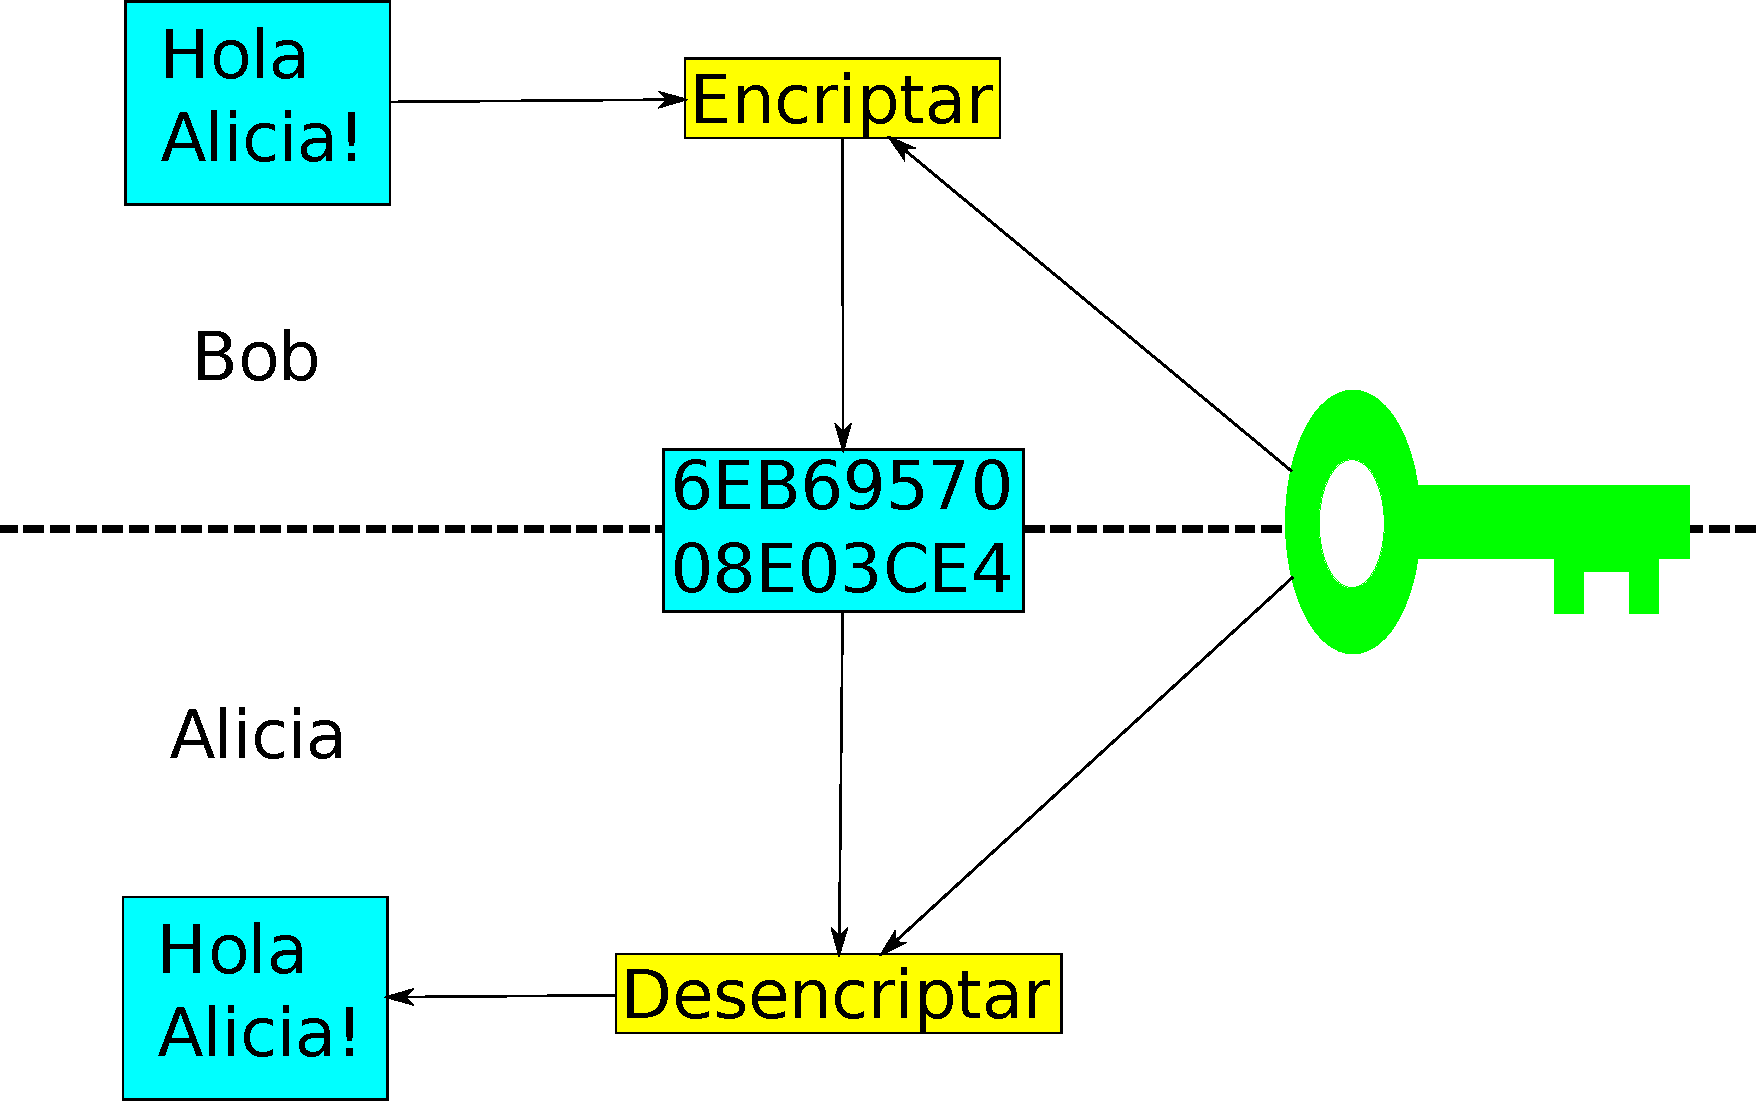
\includegraphics[scale=0.4]{Figures/SymmetricKeyEncryption}
  \decoRule
  \caption[Criptografía de clave simétrica (Esquema)]{Esquema general de la criptografía de clave simétrica}
  \label{fig:SymmetricKeyEncryption}
\end{figure}

El problema que tiene este modelo es el intercambio de las claves.
Es necesario un canal seguro por el que comunicar las claves y este tipo de algoritmos no proveen ese servicio. \emph{\parencite{Reference19}}

Es por ello que normalmente se mezcla este tipo de criptografía con otro conocido como \keyword{criptografía de clave pública}, que veremos más adelante.

%----------------------------------------------------------------------------------------

\section{Cifrado por bloques}

Dentro de la criptografía simétrica nos encontramos dos grandes algoritmos: los de \keyword{flujo} y los de \keyword{bloques}.
Nos centraremos en el segundo.

Un algoritmo basado en \keyword{cifrado por bloques} es aquel que, como su propio nombre indica,
realiza un cifrado primero dividiendo el \emph{texto plano} en bloques de un tamaño determinado\footnote{Cuando el tamaño del fichero que queremos encriptar no es múltiplo del tamaño de bloque, el bloque final tendrá un tamaño diferente al resto. Esto se soluciona con técnicas de padding, lo cual se explica en el siguiente punto.}
y luego cifrando por separado estos bloques, dando como resultado un \emph{texto cifrado}.

La mayoria de los \keyword{cifradores por bloques} son iterativos, es decir, realizan la misma operación un determinado número de veces o rondas (\emph{rounds}).
Esta operación suele ser idéntica en todas las rondas, a excepción de la primera o la última, donde suele ser distinta.

\begin{figure}[ht]
  \centering
  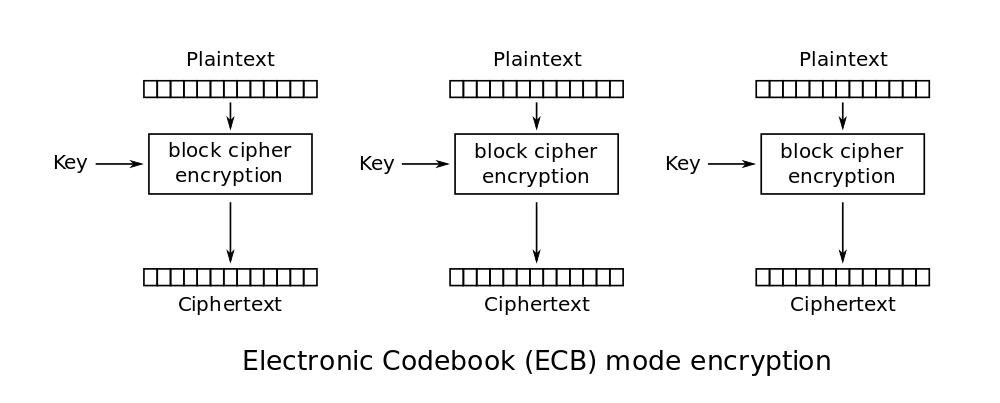
\includegraphics[scale=0.5]{Figures/ECB}
  \decoRule
  \caption[Electronic Codebook (ECB)]{Cifrado usando el modo Electronic Codebook (ECB)}
  \label{fig:ECB}
\end{figure}

Existen varios modos de operación para llevar a cabo un \keyword{cifrado por bloques}: ECB, CBC, OFB, CFB, etc.
Cada uno de ellos opera los bloque de diferente forma: algunos utilizan el bloque cifrado anterior para generar el nuevo,
otros utilizan combinaciones con estructuras del mismo tamaño que el bloque, etc. \emph{\parencite{Reference21}}

%----------------------------------------------------------------------------------------

\section{Relleno (Padding)}

\keyword{Relleno (Padding)} es el nombre que recibe la técnica que permite en criptografía por bloques expandir el último bloque del mensaje hasta lograr un tamaño deseado.

Es muy común que, en la criptografía por bloques, los fragmentos que encriptamos no tengan la longitud que queremos para nuestro sistema.
Para solucionar esto existen multitud de técnicas de \keyword{padding}, desde agregar al final del bloque un byte con un cierto valor, hasta simplemente rellenar con ceros.

El requisito indispensable que debe cumplir cualquier técnica de padding es que debe permitir al destinatario diferenciar los bytes del mensaje original de los byte de relleno. \emph{\parencite{Reference8}}

%----------------------------------------------------------------------------------------

\section{CBC}

\keyword{Cipher Block Chaining (CBC)} es uno de los modos de operación para cifrado por bloques que hemos mencionado antes,
y el que se ha decidido elegir para este proyecto.

En algunos modos como ECB, dada una clave determinada,
cualquier \emph{plaintext} siempre dará como resultado el mismo \emph{ciphertext}.
Si, como es nuestro caso, esta característica supone un problema,
se opta por otros modos de operación como CBC, el cual soluciona esto. \emph{\parencite{Reference23}}

\subsection{Modo de operación}

\keyword{CBC} funciona combinando cada bloque de \emph{plaintext} con el bloque de \emph{ciphertext} justamente anterior.
Obviamente, para el primer bloque no se dispone de un bloque cifrado anterior,
por lo que se recurre al uso de un \keyword{vector de inicialización (IV)}.
\footnote{Un IV es un conjunto de bytes aleatorios que se usan para suplir la necesidad de un bloque cifrado anterior al primer bloque.
Una muy mala práctica, por no decir prohibida, es la reutilización de un IV, ya que este debe ser de uso único.}

\begin{figure}[ht]
  \centering
  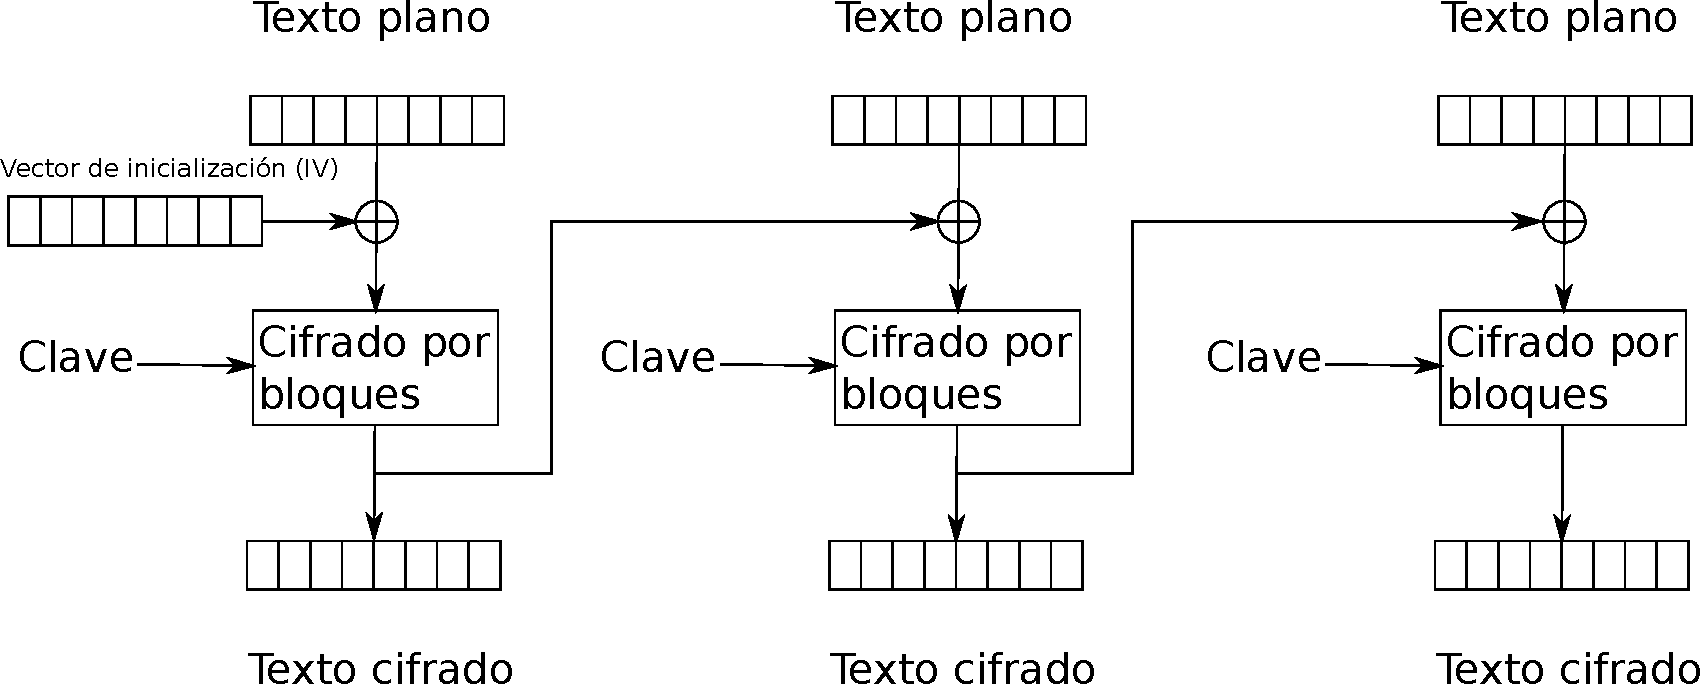
\includegraphics[scale=0.5]{Figures/CBC_enc}
  \decoRule
  \caption[Cipher Block Chaining (CBC) - Cifrado]{Cifrado usando el modo Cipher Block Chaining (CBC)}
  \label{fig:CBC_enc}
\end{figure}

Como vemos en la Figura~\ref{fig:CBC_enc}, en el cifrado con \keyword{CBC}, el primer bloque de texto y el IV son sometidos a una operación XOR.
El resultado de esta operación se pasa por una función de cifrado\footnote{La función de cifrado es la misma para todos los bloques.}, la cual nos dará el primer bloque cifrado.
Este primer bloque es entonces pasado por un XOR junto con el segundo bloque de texto, y así sucesivamente.

\begin{figure}[ht]
  \centering
  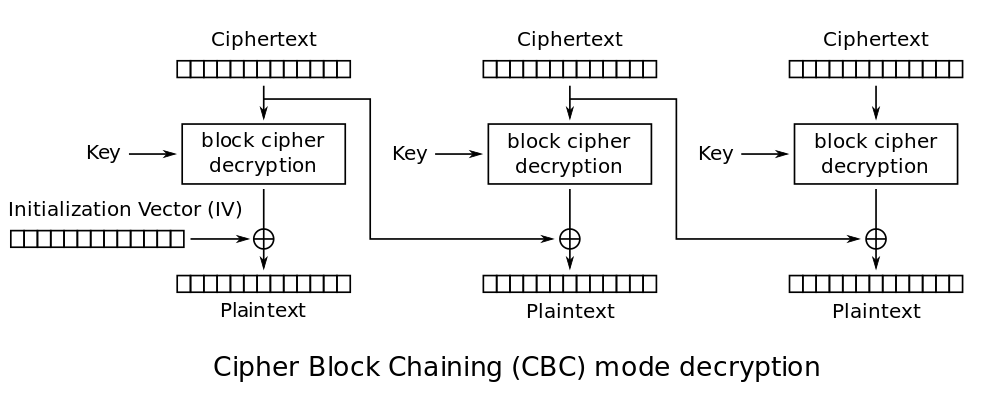
\includegraphics[scale=0.5]{Figures/CBC_dec}
  \decoRule
  \caption[Cipher Block Chaining (CBC) - Descifrado]{Descifrado usando Cipher Block Chaining (CBC)}
  \label{fig:CBC_dec}
\end{figure}

A la hora de desencriptar, la misma función utilizada en la encriptación
es usada para obtener cada bloque de texto a partir de los bloques cifrados.
Una representación de este proceso lo encontramos en la Figura~\ref{fig:CBC_dec}.

El objetivo de un \keyword{cifrado por bloques} es poder paralelizar el proceso de encriptación.
Lamentablemente, el cifrado con \keyword{CBC} debe ser secuencial,
ya que para obtener cada bloque es necesario haber generado antes el anterior.

Sin embargo, el proceso de desencriptación con \keyword{CBC} sí que puede ser paralelizado,
ya que las mútiples funciones de descifrado que se realizan no dependen de ningún bloque anterior. \emph{\parencite{Reference24}}

%----------------------------------------------------------------------------------------

\section{AES}

\label{AES}

\keyword{Advanced Encryption Standard (AES)}, también conocido como \keyword{Rijndael} por sus creadores,
es el resultado del proceso de búsqueda de un estándar para encriptación por parte del gobierno de los Estados Unidos.

\keyword{AES} es una variante de \keyword{Rijndael} (que a su vez es una variante de Square), del cual solo toma algunos modos.
Mientras que el algoritmo original puede tomar tamaños de bloque múltiplos de 32 bits,\footnote{Con un mínimo de 128 bits y un máximo de 256.}
\keyword{AES} únicamente opera con tamaños de bloque igual a 128 bits.

Con el tamaño de las claves ocurre algo parecido, ya que \keyword{AES} solo soporta tamaños de 128, 192 y 256 bits,
mientras que el algoritmo original soporta unos cuantos más. \emph{\parencite{Reference25}}

\subsection{Estado (State)}

Antes de meternos a hablar del algoritmo en sí, es necesario explicar una estructura que se usará
constantemente.

El \keyword{Estado (State)} es una estructura bidimensional de bytes con la que se operan los bytes
de los bloques de entrada. Está compuesto por 4 filas y 4 columnas, dando un total de 32 celdas,
en las cuales se almacenan los 16 bytes que forman un bloque. \emph{\parencite{Reference26}}

\subsection{Transformaciones}

El algoritmo consta de ciertas fases, una de ellas consiste en someter el \emph{State}
a unas cuantas rondas de transformaciones. Estas transformaciones son las siguientes:

\begin{itemize}
  \item \keyword{SubBytes} -- Mediante una transformación no lineal,
  los bytes del \emph{State} son reemplazados por otros usando una tabla de sustitución.
  (Figura~\ref{fig:SubBytes})

  \item \keyword{ShiftRows} -- Los bytes de las 3 últimas filas del \emph{State}
  se desplazan de manera cíclica, cada fila con un offset distinto.
  (Figura~\ref{fig:ShiftRows})

  \item \keyword{MixColumns} -- Mediante una transformación lineal,
  las columnas del \emph{State} se mezclan para producir unas nuevas.
  (Figura~\ref{fig:MixColumns})

  \item \keyword{AddRoundKey} -- En esta transformación, una \emph{Round Key} se
  añade al \emph{State} mediante una operación XOR.
  La itud de la \emph{Round Key} debe ser igual al tamaño del \emph{State}.
  (Figura~\ref{fig:AddRoundKey})
\end{itemize}

\begin{figure}[ht]
  \centering
  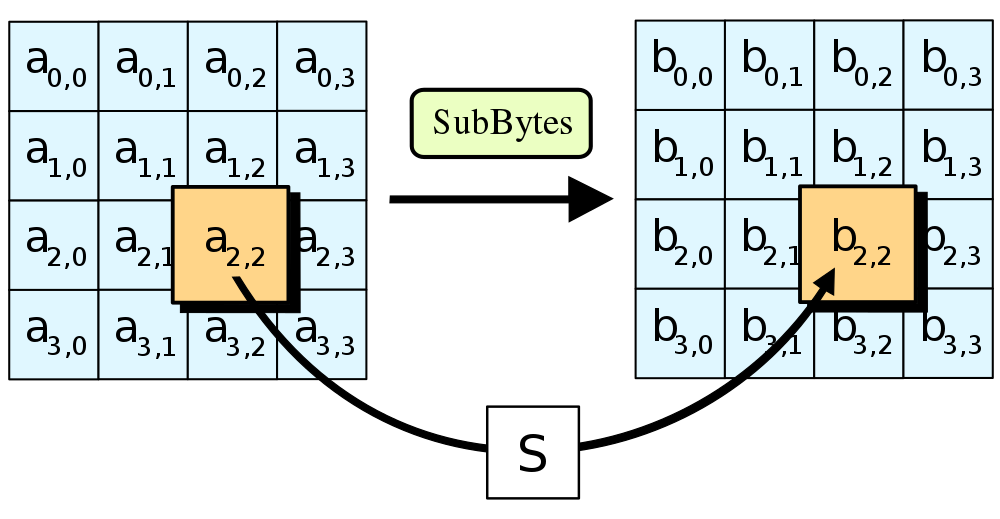
\includegraphics[scale=0.25]{Figures/SubBytes}
  \decoRule
  \caption[SubBytes (AES)]{Operación SubBytes para AES \emph{\parencite{Reference27}}}
  \label{fig:SubBytes}
\end{figure}

\begin{figure}[ht]
  \centering
  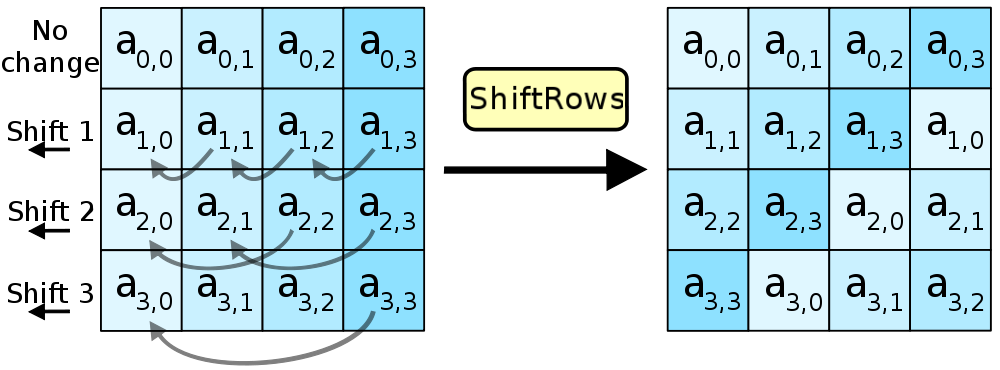
\includegraphics[scale=0.25]{Figures/ShiftRows}
  \decoRule
  \caption[ShiftRows (AES)]{Operación ShiftRows para AES \emph{\parencite{Reference28}}}
  \label{fig:ShiftRows}
\end{figure}

\begin{figure}[ht]
  \centering
  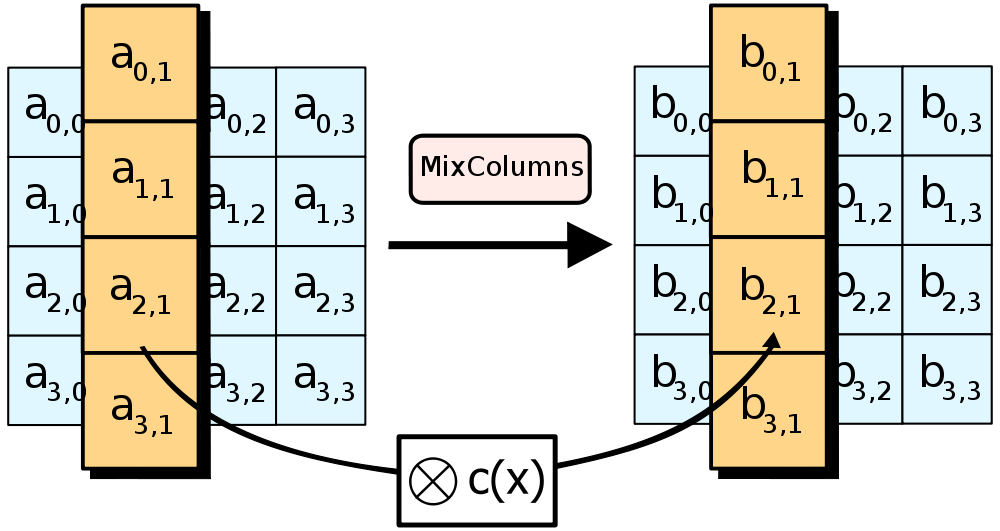
\includegraphics[scale=0.25]{Figures/MixColumns}
  \decoRule
  \caption[MixColumns (AES)]{Operación MixColumns para AES \emph{\parencite{Reference29}}}
  \label{fig:MixColumns}
\end{figure}

\begin{figure}[ht]
  \centering
  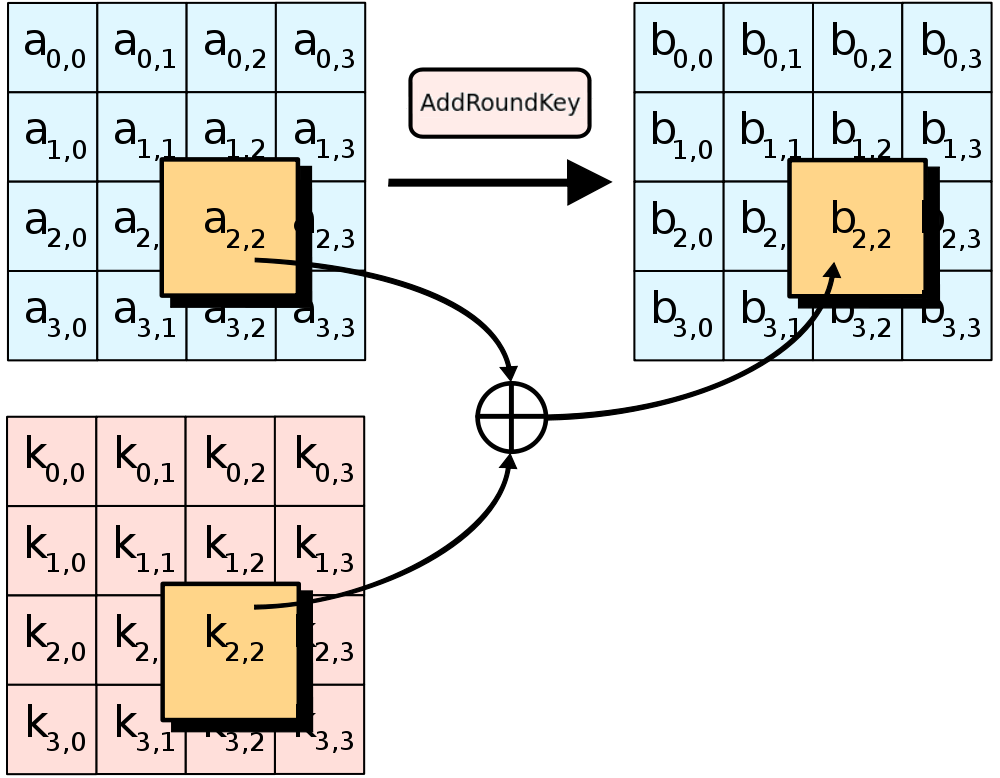
\includegraphics[scale=0.25]{Figures/AddRoundKey}
  \decoRule
  \caption[AddRoundKey (AES)]{Operación AddRoundKey para AES \emph{\parencite{Reference30}}}
  \label{fig:AddRoundKey}
\end{figure}

\emph{\parencite{Reference26}}

\subsection{Algoritmo}

En \keyword{AES} el tamaño del bloque de entrada, del de salida y del \emph{State} es de 128 bits,
y el tamaño de la clave puede tomar los valores de 128, 192 ó 256 bits.

Para cada bloque de entrada, la primera etapa del algoritmo consiste en generar las \emph{Round Keys} a partir de la clave,
usando el esquema de claves Rijndael.\footnote{Este esquema expande una clave en un número determinado de claves separadas.}

Una vez conseguidas las \emph{Round Keys}, se pasa por una ronda inicial especial
en la cual solo se realiza la transformación \emph{AddRoundKey}.

\begin{table}[ht]
  \caption{Combinaciones para el número de rondas en AES.}
  \label{tab:rounds}
  \centering
  \begin{tabular}{l l l}
  \toprule
  \tabhead{Key size (bits)} & \tabhead{Block size (bits)} & \tabhead{Rounds (Nr)} \\
  \midrule
  128 & 128 & 10\\
  192 & 128 & 12\\
  256 & 128 & 14\\
  \bottomrule\\
  \end{tabular}
\end{table}

Después de esta etapa inicial, se pasa a las rondas habladas en el punto anterior.
El número de rondas que lleva a cabo el algoritmo depende del tamaño de la clave,
lo cual vemos representado en el Cuadro~\ref{tab:rounds}.

En todas estas rondas menos en la útlima, el orden de las transformaciones será siempre el mismo:
\[ SubBytes \rightarrow ShiftRows \rightarrow MixColumns \rightarrow AddRoundKey \]

La última ronda es idéntica a las anteriores salvo por el hecho de que la transformación \emph{MixColumns} no se realiza.

El resultado de todo esto será el \emph{output} de nuestro bloque de entrada. \emph{\parencite{Reference26}}

%----------------------------------------------------------------------------------------

\section{Criptografía de clave pública}

Uno de los problemas que tiene la \keyword{criptografía de clave simétrica} es que usamos la misma clave para el cifrado y el descifrado, por lo que se hace necesaria su ocultación.
En la \keyword{criptografía de clave pública}, al hacer uso de dos claves, no es necesario mantener en secreto ambas. Aquella que ocultamos es llamada clave privada y la otra, pública.

La esencia de este algoritmo radica en que un mensaje cifrado con una clave pública solo puede ser descifrado con su homóloga privada, y viceversa.
De esta manera podemos, tal como su propio nombre indica, difundir públicamente nuestra clave \emph{pública} mientras mantenemos oculta la \emph{privada}.

Si lo que queremos es \emph{confidencialidad} durante la comunicación, entonces encriptaremos el contenido del mensaje con la clave pública del destinatario, de forma que solo él podrá descifrarlo (Figura~\ref{fig:PublicKeyEncryption}).

Por otra parte, también nos interesa que cuando alguien reciba nuestro mensaje pueda estar seguro de que realmente es nuestro.
Para lograr esto, lo que hacemos es cifrar un resumen del mensaje (\emph{hash}) con nuestra clave privada.
De esta forma, cuando alguien lo descifre con nuestra clave pública y compruebe el resumen, podrá estar seguro de que proviene de nosotros.\footnote{Es, en esencia, el fundamento sobre el que se basa la firma digital.}
Así conseguimos preservar la \emph{integridad} y la \emph{autentificación} del mensaje, dos parámetros muy importantes a tener en cuenta en seguridad. \emph{\parencite{Reference14}}

\begin{figure}[ht]
  \centering
  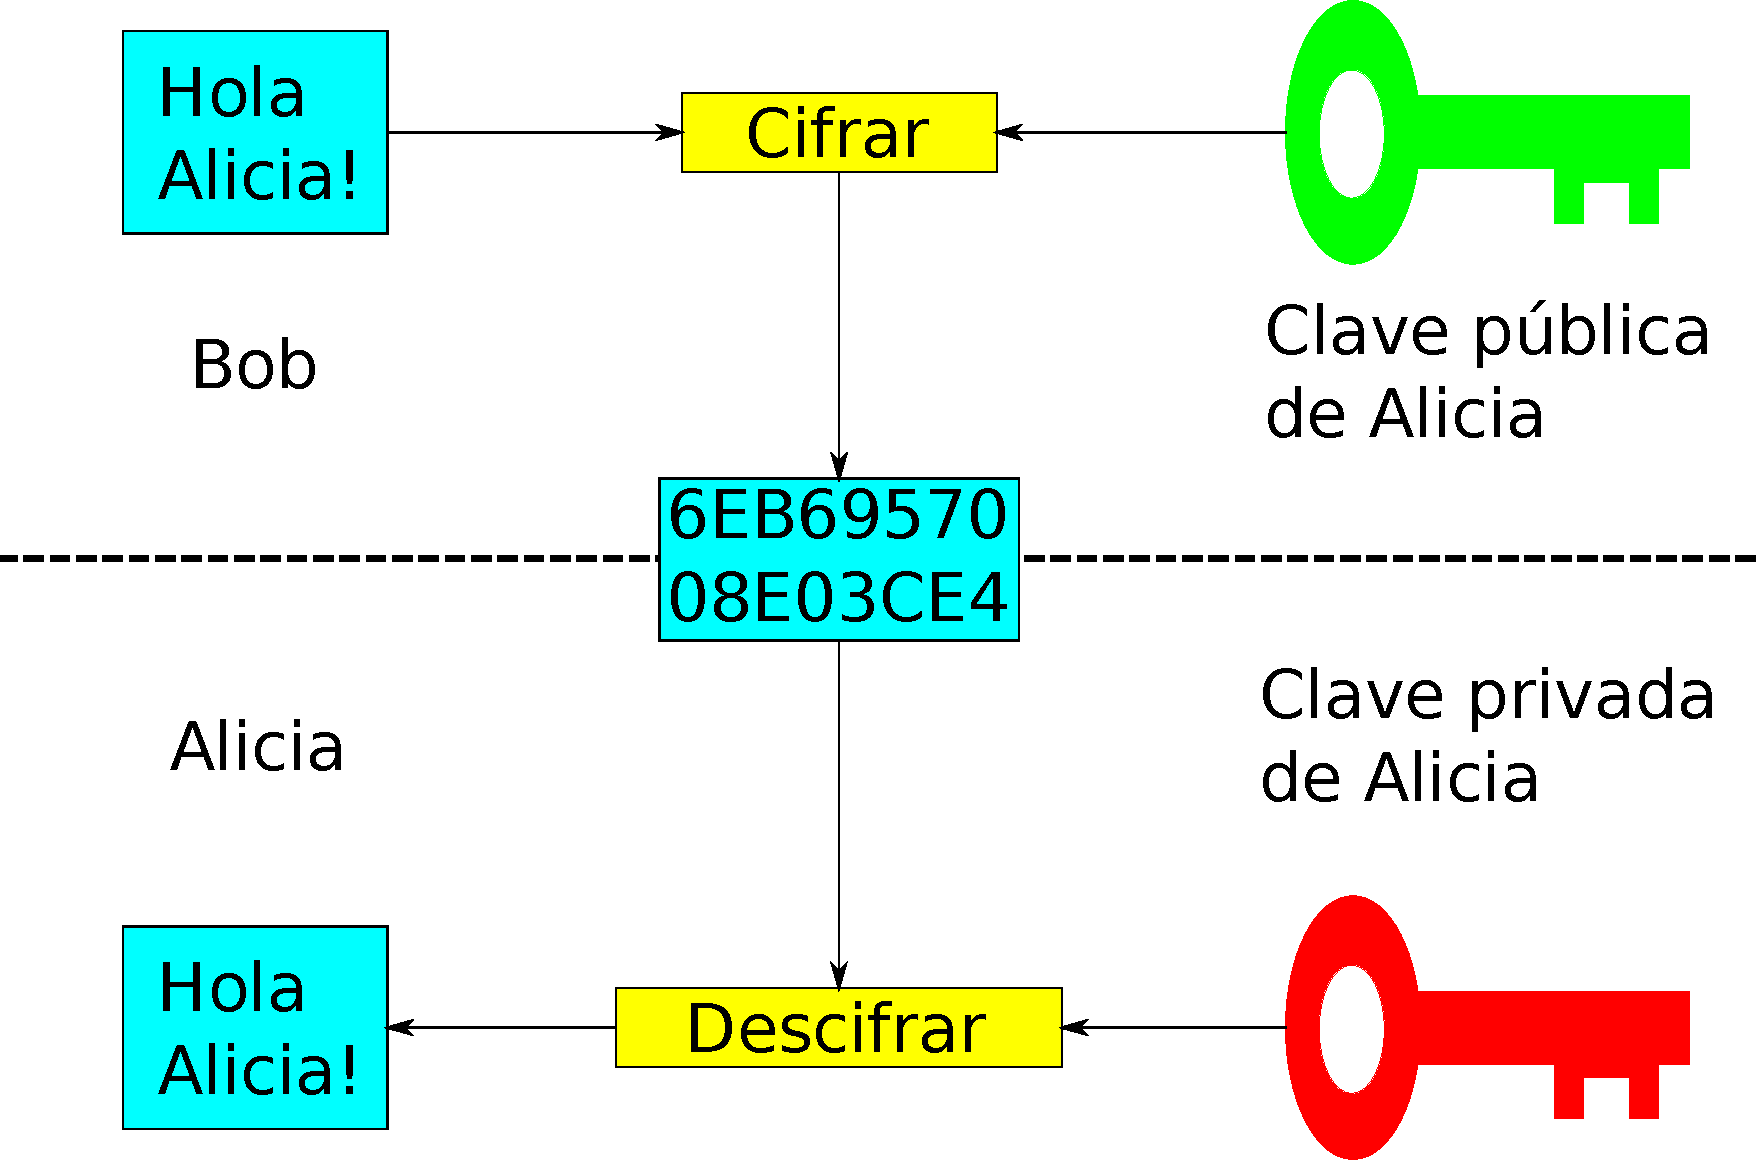
\includegraphics[scale=0.3]{Figures/PublicKeyEncryption}
  \decoRule
  \caption[Cifrado de clave pública (Esquema)]{Esquema general del cifrado de clave pública}
  \label{fig:PublicKeyEncryption}
\end{figure}

%----------------------------------------------------------------------------------------

\section{RSA}

\label{RSA}

Uno de los primeros algoritmos de criptografía pública (y el más utilizado hoy) es \keyword{RSA} (\keyword{Rivest–Shamir–Adleman})\footnote{RSA debe su nombre a sus creadores: Ron Rivest, Adi Shamir y Leonard Adleman.}.
Una de sus características más distintivas es el problema que plantea factorizar el producto de dos grandes números primos (\emph{factoring problem}).
El resultado de esta factorización es luego usado en la generación de las claves.

En general, los algortimos de criptografía de clave pública son bastante más lentos que los de clave simétrica.
Por ello, se suelen usar en conjunto con algún algoritmo de criptografía simétrica, como \keyword{AES}. \emph{\parencite{Reference9}}

\subsection{Clave pública RSA}

Dentro del conjunto del par de claves \keyword{RSA}, la \emph{pública} es aquella que no mantenemos en secreto para que cualquiera que quisiera comunicarse con nosotros pudiera hacerlo de manera confidencial.
Este tipo de claves consta de dos elementos:
\begin{itemize}
  \item \keyword{n} -- el módulo RSA, un entero positivo.
  \item \keyword{e} -- el exponente público RSA, otro entero positivo.
\end{itemize}

Lo primero que se debe hacer para generar la clave \emph{pública} es seleccionar de manera aleatoria dos números primos impares distintos, lo suficientemente grandes como para que sea computacionalmente inviable su descubrimiento por parte de un atacante.
Una vez encontrados, el módulo \keyword{n} de la clave \emph{pública} será el producto de estos dos números primos.\footnote{Por convención, se denotan como \emph{p} y \emph{q}.}
\[ n = p \boldsymbol{\cdot} q \]

Ahora que tenemos el módulo de la clave definido, es hora de generar un exponente público \keyword{e} adecuado.
Para ello, haremos uso de la función de Carmichael\footnote{La función que se muestra solo es válida cuando n es el producto de dos números primos impares y distintos.}, la cual tiene la siguiente forma:
\[ \lambda(n) = mcm(p - 1, q - 1) \]
El exponente público \keyword{e} será aquel número entero comprendido entre 3 y (\keyword{n} - 1) que satisfaga:
\[ MCD(e, \lambda(n)) = 1 \] \emph{\parencite{Reference10}}

\subsection{Clave privada RSA}

La clave \emph{privada} es la que mantenemos oculta. Aunque existen varios modelos, generalmente consta de dos elementos:
\begin{itemize}
  \item \keyword{n} -- el módulo RSA, un entero positivo (Debe ser el mismo que el de la clave \emph{pública}).
  \item \keyword{d} -- el exponente privado RSA, un entero positivo.
\end{itemize}

Para calcular el exponente privado \keyword{d} deberemos elegir un entero positivo menor que \keyword{n}, que además cumpla:
\[ e \boldsymbol{\cdot} d \equiv 1 \Mod{\lambda(n)} \]
, donde \keyword{e} será el correspondiente exponente público. \emph{\parencite{Reference11}}

\subsection{Evaluación de la función RSA}

Lo primero que debemos hacer es conseguir una representación de nuestro mensaje como un número entero, comprendido entre 0 y (\keyword{n} - 1).

Vamos a suponer que este mensaje queremos enviárselo a alguien cuya clave pública es (\emph{e, n}).
Si nuestro mensaje (recordemos que ahora es un entero) es \emph{M}, para obtener el mensaje cifrado, aplicaremos la siguiente operación:
\[ C \equiv E(M) \equiv M^e \Mod{n} \]
El entero \emph{C} será del mismo tamaño que \emph{M} y representará al mensaje cifrado.

Si ahora el destinatario quisiera descifrar el mensaje, solo tendría que revertir la operación con su clave privada (\emph{d, n}) de la siguiente manera:
\[ M \equiv D(C) \equiv C^d \Mod{n} \]
De esta manera, recuperaría el mensaje original.\footnote{Para cifrar con una clave privada y descifrar con una pública se hacen las mismas operaciones, cambiando e y d donde corresponda.} \emph{\parencite{Reference12}}

%----------------------------------------------------------------------------------------

\section{RSASSA-PSS}

\label{RSASSA-PSS}

Antes hablamos de la necesidad de preservar la \emph{integridad} y la \emph{autentificación} en las comunicaciones.
\keyword{RSASSA-PSS} es un algoritmo de firma digital que sirve precisamente para ello.
Combina RSA con un método de codificación llamado Probabilistic Signature Scheme (PSS).
\footnote{Las siglas SSA corresponden a Signature Scheme with Appendix, lo que quiere decir que la firma va añadida al final del mensaje o junto a él.}

\subsection{\emph{Salt}}

En criptografía, una \keyword{\emph{salt}} es un fragmento de bits aleatorios
que se utiliza junto a claves, funciones hash y otros mecanismos de cifrado con
el fin de prevenir ataques de diccionario o de \emph{rainbow table}.
\emph{\parencite{Reference32}}

\subsection{HMAC}

\label{HMAC}

Una \keyword{HMAC} (\keyword{Hash-based Message Authentication Code}) es una
construcción usada para verificar la integridad de un mensaje, así como a su
autor.

Hace uso de una función hash criptográfica, como MD5 o SHA-1, junto a una clave
criptográfica secreta. La robustez de una HMAC depende de la función hash
elegida, del tamaño del resumen y del tamaño de la clave.
\emph{\parencite{Reference31}}

\subsection{Probabilistic Signature Scheme (PSS)}

\label{PSS}

\keyword{PSS} es un método de codificación\footnote{Un método de codificación es una operación que permite convertir un carácter de un determinado conjunto en un símbolo de otro sistema de representación.}
desarrollado por Mihir Bellare y Phillip Rogaway, los cuales buscaban mejorar los métodos que existían.
Para ello, incluyeron en su esquema el uso de una \emph{salt}, lo cual haría más seguro el algoritmo frente a intentos de romperlo. \emph{\parencite{Reference15}}

\begin{figure}[ht]
  \centering
  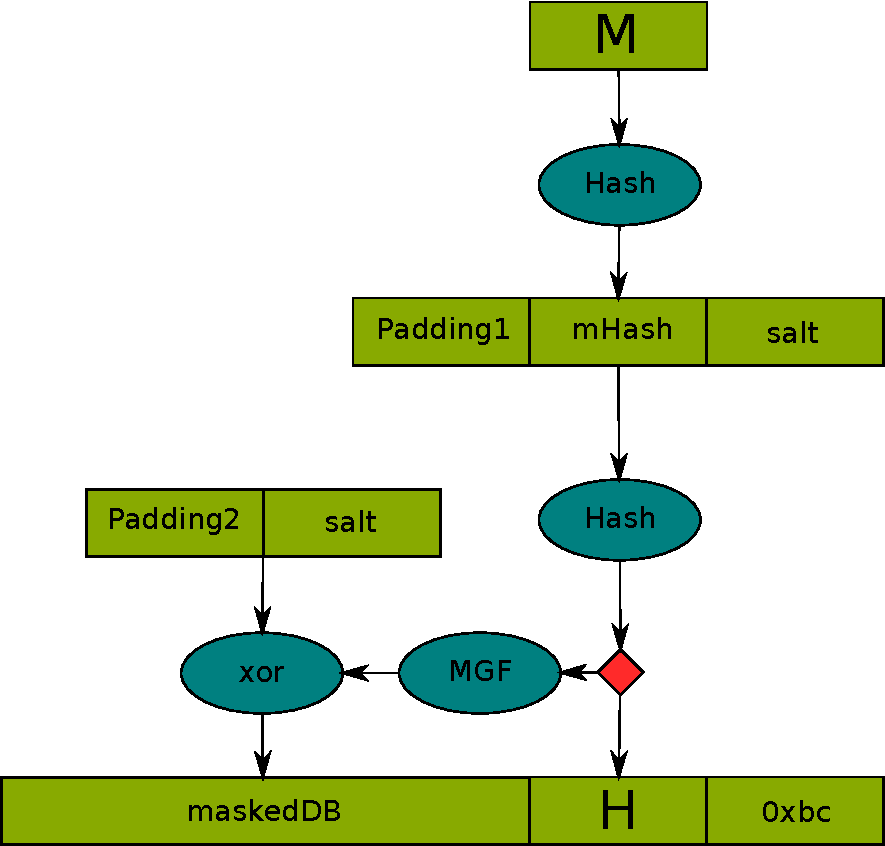
\includegraphics[scale=0.6]{Figures/PSS}
  \decoRule
  \caption[PSS (Esquema)]{PSS de acuerdo a PKCS \#1 V2.2 / RFC 8017}
  \label{fig:PSS}
\end{figure}

Como vemos en la Figura~\ref{fig:PSS}, \keyword{PSS} genera un resumen (\emph{hash}) del mensaje.
Este resumen se vuelve a pasar de nuevo por una función \emph{hash}\footnote{Las dos funciones \emph{hash} que se usan en el esquema deben ser la misma.}
junto a un \emph{padding}\footnote{El primer \emph{padding} estará formado por 8 bytes con valor \emph{0x00}.} y la \emph{salt} tal como muestra la figura.

El resultado de esta operación será la segunda de 3 piezas que conformarán nuestro mensaje codificado y la denotaremos como \keyword{H}.
Para la primera (\emph{maskedDB}), generaremos una máscara\footnote{Una máscara es muy parecida a una \emph{hash}. Mientras la segunda tiene un tamaño determinado, una máscara puede tomar distintos tamaños según la necesidad.} de \keyword{H} y haremos una operación \emph{xor} con ella y la salt (junto a otro \emph{padding}).\footnote{Este \emph{padding} está formado por una cantidad variable de bytes con valor \emph{0x00}, teniendo al final un byte de valor \emph{0x01}.}

Ahora solo nos quedará añadir al final de nuestra salida un byte con valor \emph{0xbc} y ya habremos acabado. \emph{\parencite{Reference17}}

%----------------------------------------------------------------------------------------

\section{HTTP}

\keyword{Hypertext Transfer Protocol (HTTP)} es un protocolo de nivel de aplicación
para sistemas de información distribuidos.

Es un protocolo genérico y sin estado que es usado para múltiples tareas como
la transferencia de hipertexto o la representación de sistemas de ficheros.

Una característica de HTTP es la negociación de la representación de los datos,
lo que permite construir sistemas indpendientemente de los datos que se vayan a
transmitir. \emph{\parencite{Reference18}}
